%\chapter{Flux de données: flux{\_}vls (PAU)}
\chapter{Spécifications}
\section{Spécification fonctionnelle}
\subsection{Présentation}
Nous nommons flux{\_}vls l'ensemble des applications gérant les différents processus allant de l'obtention des données jusqu'à l'agrégation des données stockées. Les données sont les valeurs liquidatives datées des fonds trouvés. Nous appelons fonds un portefeuille de titres géré par un professionnel et proposé par un établissement financier ou une banque. Flux{\_}vls est donc composé d'un processus d'obtention des données, un processus d'intégration des données et un processus d'agrégation et de préparation des données. Il existe aussi un processus chargé de la maintenance de la base ou du moins ce qui peut être traité de manière automatique.
\subsection{Processus d'obtention des données}
Nous appelons donnée le tuple $\lbrace ISIN\protect\footnote{International Securities Identification Number}, devise, VL\protect\footnote{Valeur Liquidative}, date\ de\ la\ valorisation \rbrace$. L'isin est un code à 12 caractères permettant d'identifier les valeurs de manière internationale.\\
Les données sont obtenues par robot web.\\
Chaque soir le processus lance un robot web par fournisseur agrégé \textit{(voir la liste des fournisseurs agrégés \ref{fournisseurs} page~\pageref{fournisseurs})}.\\
Le robot web se connecte au site web du fournisseur.\\
Le robot web met les données au format {\og}$ISIN;DEV;VL(ex:10.00);jj/mm/aaaa${\fg}  dans un fichier textué.\\
Le robot web crée donc un fichier par fournisseur.\\
Un robot web supplémentaire est destiné à obtenir les taux de conversion DEV$\rightarrow$EUR avec le format {\og}$DEV;jj/mm/aaaa;taux(ex:10.00)${\fg}  de manière à ce qu'on ait $1 EUR = taux \times DEV$.

\subsection{Processus d'intégration des données et base de données associée}
Les fichiers créés par le processus d'obtention des données sont ouverts un par un et leur contenu est stocké dans une base de données appellée flux{\_}vls.
Le processus vérifie que les données ne sont pas trop absurdes.
On entend par absurde le fait qu'un tuple candidat à l'insertion ne vérifie pas le bon format ou que la date de la valeur soit supérieure à la date du jour.

\subsection{Processus d'agrégation et de préparation des données, base de données associée et calcul des taux d'évolution}
L'ensemble des données stockées dans flux{\_}vls est par ce processus restreint à l'ensemble des données qui concernent CYRUS CONSEIL (soit $\approx$ 1 000 fonds). Les données qui concernent CYRUS CONSEIL sont les valeurs des supports dont le montant souscrit est supérieur à 0 et possédant un ISIN. La discrimination se fait à partir de la base du système d'informations ajourd'hui appelée BDD8DEFSQL.\\ 
La base de données contenant les données restreintes sera appelée flux{\_}vls{\_}eur. flux{\_}vls{\_}eur est différente de la base contenant la totalité des données. Ainsi, si BDD8DEFSQL comporte des informations erronnées, la contamination ne se propage que dans flux{\_}vls{\_}eur. flux{\_} est ainsi protégée de toute contamination externe.\\
Les calculs des taux d'évolution s'effectuent à partir de flux{\_}vls{\_}eur. De cette manière on ne fait des calculs que pour les fonds dont on a besoin. Cela permet de diminuer le temps de calcul qui est déjà très long (5 heures). Le résultat des calculs est stocké dans une table prête à servir facilement.

\subsection{Processus de maintenance de la base}
Il existe un processus lancé quotidiennement qui sauvegarde et archive flux{\_}vls et flux{\_}vls{\_}eur. Il est normalement fait un vacuum. Il faudrait ajouter à cela un réindexage total lancé de manière bimensuelle. Il existe un outil pour créer une table de performances arrêtées à une date.
\clearpage
\section{Rôle et identification des différents fichiers}
\subsection{Présentation}
Nous allons dans cette section décire les différents fichiers intervenant dans le flux de valeurs liquidatives. Pour les bases de données on donnera simplement le diagramme.
\subsection{Bases de données}
\subsubsection{Base de données flux{\_}vls}
	\begin{changemargin}{-2.5cm}{-1cm}
		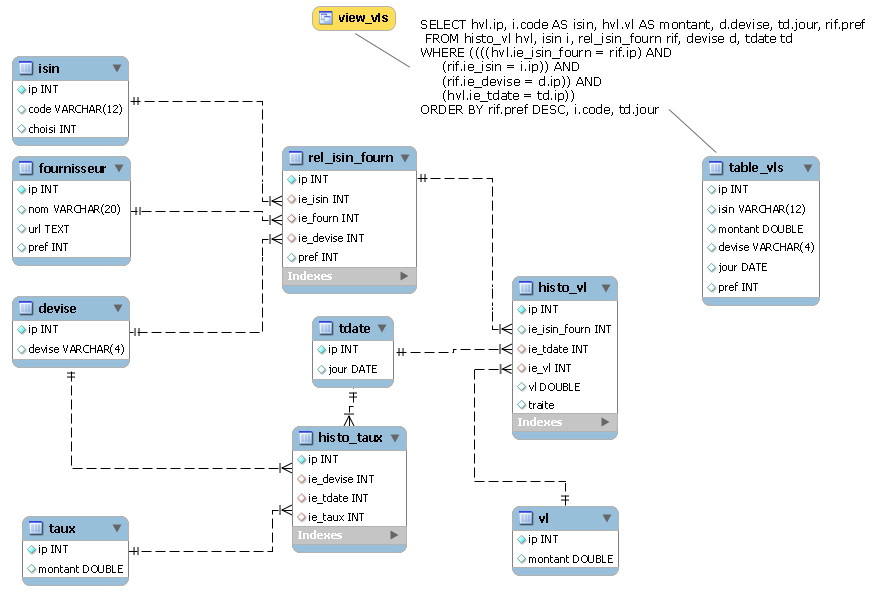
\includegraphics[scale=0.6]{images/flux_vls_map.png} 
	\end{changemargin}
	\clearpage
\subsubsection{Base de données flux{\_}vls{\_}eur}
	\begin{changemargin}{-2.5cm}{-1cm}
		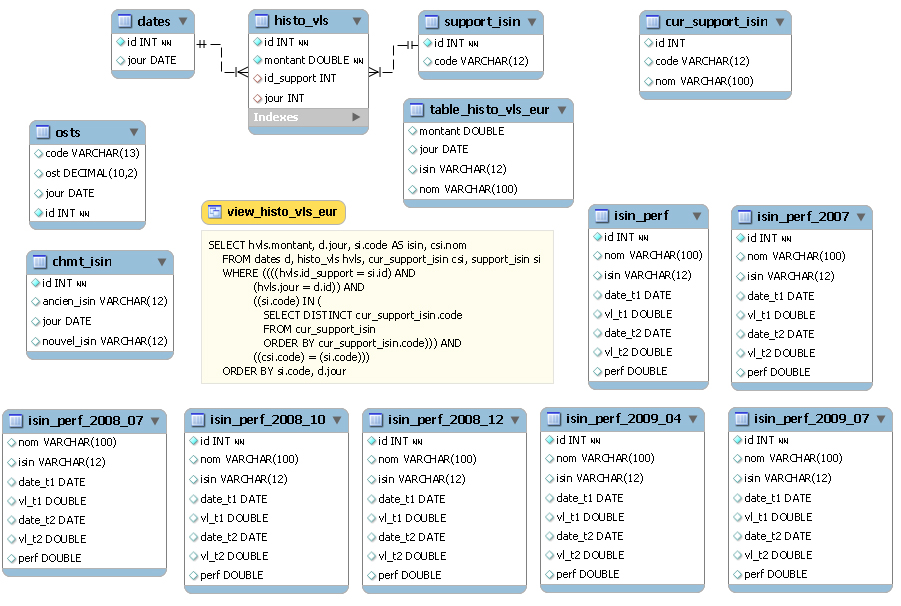
\includegraphics[scale=0.6]{images/flux_vls_eur_map.png} 
	\end{changemargin}	
\subsubsection{Programmes}
\paragraph{/home/postgres/db/script/do{\_}back{\_}up.sh} Lancé par le cron de postgres quotidiennement.\\
Ici, {\$}TODAY représente la date du jour. {\$}TODAY est déterminé avec la commande bash :
\lstset{language=bash}
\begin{lstlisting}
 `date +"{\%}Y{\%}m{\%}d-{\%}H"`
\end{lstlisting}
Ce que fait le fichier : 
\begin{enumerate}
\item Crée un répertoire /home/postgres/db/backup/{\$}TODAY,
\item Sauvegarde la base de données flux{\_}vls dans le fichier flux{\_}vls{\$}TODAY.sql via pg{\_}dump,
\item Sauvegarde la base de données flux{\_}vls{\_}eur dans le fichier flux{\_}vls{\_}eur{\$}TODAY.sql via pg{\_}dump,
\item Le répertoire {\$}TODAY est {\og}taré{\fg}  et {\og}gzipé{\fg}  via tar -cvzf,
\item Le serveur de bases de données est redémarré.
\end{enumerate}
\paragraph{/home/malko/flux{\_}vls/outils/create{\_}isin{\_}perf{\_}arretee.rb} \label{arret-perf}Lancé manuellement avant chaque génération des états de compte.\\
Ce programme crée une table de la forme : isin{\_}perf{\_}yyyy{\_}mm avec yyyy{\_}mm l'année (2009 par exemple) et le mois (07 par exemple).\\
Ce programme s'utilise comme suit :\\
La table de performances arrêtées se crée le 02 ou le 03 du mois pour avoir les données du 1\up{er} du mois.
\begin{enumerate}
\item Se connecter sur la machine du flux (actuellement prodserver : 192.168.0.78),
\item Aller dans \path{/home/malko/flux_vls/outils},
\item ruby create{\_}isin{\_}perf{\_}arretee.rb,\\
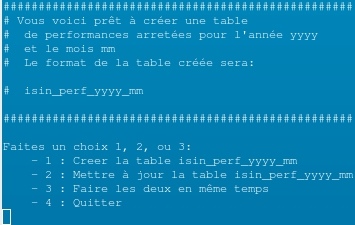
\includegraphics[clip=true, width=335px, height=225px]{./images/creation.jpg}\\
\item Choisir 3 dans la plupart des cas,
\item Suivre ce qui est indiqué.
\end{enumerate}
	\clearpage
\subsection{Processus d'obtention des données}
Dans la suite de ce document nous appelons \path{#} \path{/home/malko/flux_vls/}.\\
\subsubsection{Programmes}
\paragraph{{\#}/imports/import{\_}vl.sh} Lancé par le cron.
\begin{itemize}
\item Création du fichier \path{#/imports/a_import.py} par le script \path{#/imports/creation_fichier_import.py}.\\
Du code python est créé pour gérer chaque robot.\\
Exemple du code créé dans le fichier a{\_}import.py (ici gestion du robot cardif): \\
\lstset{language=python, keywordstyle=\color{Ror}}
\lstset{frame=shadowbox, rulesepcolor=\color{Ror}}
\begin{lstlisting}
import os
import datetime
import fournisseurs.import_cardif
global repertoire_fichiers
repertoire_fichiers = '/home/malko/flux_vls/fichiers/'
def file_exists(fichier):
    try:
        file(fichier)
        return True
    except:
        return False
if file_exists('log/imports.log'):
    os.remove('log/imports.log')
file_log = open('log/imports.log', 'a')
try:
    print "debut " + "cardif"
    fournisseurs.import_cardif.import_cardif()
except Exception, e:
    print "!!!!!!!!!!!!!!cardif a plante"
    print e
    fichier = '/home/malko/flux_vls/imports/' +
	'fournisseurs/import_cardif.py\n'
    file_log.write(fichier)
file_log.close()
\end{lstlisting}
\item Lancement du script \path{#/imports/a_import.py}.\\
	L'historique des évènements s'enregistre dans le fichier \path{#/imports/log/imports.log}.\\
	Ce script lance les robots.
\item Lancement de \path{#/import_ds_bdd.rb}
\end{itemize}
\paragraph{robots}
\label{robots}
Les robots sont dans le répertoire \path{#/imports/fournisseurs/}. Un robot a comme nom de fichier import{\_}fournisseur.py où fournisseur est le nom du fournisseur. Un robot peut avoir aussi un fichier import{\_}fournisseur.rb mais il faut impérativement qu'il y ait un fichier import{\_}fournisseur.py. Un fichier python contient obligatoirement une méthode comme : 
\lstset{language=python, keywordstyle=\color{Ror}}
\lstset{frame=shadowbox, rulesepcolor=\color{Ror}}
\begin{lstlisting}
def import_fournisseur():
	#code du robot ou 
	#appel du robot ruby import_fournisseur.rb
\end{lstlisting}
Les robots utilisent les fichiers \path{#/imports/fournisseurs/support.py} pour les robots entièrement en python et \path{#/imports/fournisseurs/support.rb} pour les robots mi--python/mi--ruby. Ces fichiers contiennent les classes $Support(isin, devise, vl, date)$.\\
Le robot morningstar est particulier : il se trouve dans le répertoire \path{#/imports/fournisseurs/robot_morningstar} et est lancé séparément par son propre cron.
\paragraph{{\#}/imports/manage{\_}robot.sh}
Ce que fait ce script :
\begin{itemize}
	\item Efface les fichiers python et ruby du fournisseur.
		Pour créer les fichiers python et ruby il faut avoir enlevé du répertoire \path{#/imports/fournisseurs/} les fichiers \path{import_fournisseur.py} et \path{import_fournisseur.rb} car on veut être sûr de ne pas supprimer un fichier par inadvertance.
	\item Crée les fichiers python et ruby nécessaires au robot fournisseur à partir des modèles \path{#/imports/fournisseurs/modele/import_modele.[py|rb]}.
	\item Ouvre les fichiers python et ruby du robot fournisseur.	
\end{itemize}
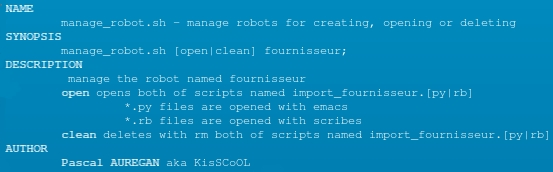
\includegraphics[clip=true, width=500px, height=150px]{./images/robot.jpg}\\
\paragraph{{\#}/fichiers/import{\_}fournisseur.txt $\vert$ taux{\_}ecb.txt}
\label{fichiers-flux}
Ce sont les fichiers produits par les robots.
Ces fichiers sont importés puis archivés.\\
Exemple de fichier import{\_}fournisseur.txt
\lstset{language=python, keywordstyle=\color{Ror}}
\lstset{frame=shadowbox, rulesepcolor=\color{Ror}}
\begin{lstlisting}
FR0010129114;63.07;EUR;28/07/2009
\end{lstlisting}
Exemple de fichier taux{\_}ecb.txt :
\lstset{language=python, keywordstyle=\color{Ror}}
\lstset{frame=shadowbox, rulesepcolor=\color{Ror}}
\begin{lstlisting}
LTL;30/07/2009;3.4528
\end{lstlisting}

\subsubsection{Fichiers logs}
\paragraph{{\#}/imports/log/imports.log}
La partie de ce fichier qui nous intéresse ici est la partie liée aux téléchargements des robots. Lorsque un robot plante, une première indication est écrite.\\
Exemple d'une ligne de log pour ecofi :
\lstset{language=python, keywordstyle=\color{Ror}}
\lstset{frame=shadowbox, rulesepcolor=\color{Ror}}
\begin{lstlisting}
debut ecofi
"ECOFI:::FR0010706549::: non trouve"
\end{lstlisting}
\paragraph{{\#}/imports/log/log{\_}sp.log}
On trouve dans ce fichier les liens morningstar visités.
\subsection{Processus d'intégration des données}
\subsubsection{Programmes}
\paragraph{{\#}/import{\_}ds{\_}bdd.rb}
Ce programme importe les fichiers présents dans \path{#/fichiers/}. Les taux taux{\_}ecb.txt sont importés en premier. Les fichiers import{\_}fournisseur.txt sont importés ensuite.
\paragraph{{\#}/imports/backup{\_}import{\_}files{\_}bdd.rb}
Ce programme archive dans \path{#/fichiers/backup} les fichiers présents dans \path{#/fichiers/}. Les archives créés à partir de {\og}tar -cvzf{\fg}  se nomment sous la forme yyyymmdd-hh.tgz où yyyy, mm, dd, hh représentent respectivement l'année (ex : 2009), le mois (ex : 05 pour le mois de Mai), le jour (ex : 31) et l'heure (ex : 02 pour 2 heures du matin).
\subsubsection{Fichiers logs}
\paragraph{{\#}/imports/log/imports.log}
\subparagraph{{\#}/import{\_}ds{\_}bdd.rb}
Exemple pour l'import d'ecofi:
\lstset{language=python, keywordstyle=\color{Ror}}
\lstset{frame=shadowbox, rulesepcolor=\color{Ror}}
\begin{lstlisting}
::2009-08-01 08:59 => updating database...
"00:48 => debut ecofi"
"00:50 => fin ecofi"
::2009-08-01 08:59 => database updated
\end{lstlisting}
\subparagraph{{\#}/imports/backup{\_}import{\_}files{\_}bdd.rb}
Exemple de sauvegarde :
\lstset{language=python, keywordstyle=\color{Ror}}
\lstset{frame=shadowbox, rulesepcolor=\color{Ror}}
\begin{lstlisting}
::2009-08-01 02:43 => changing directory to 
	/home/malko/flux_vls/imports/ successed
::2009-08-01 02:43 => creating 20090801-02 directory ...
::2009-08-01 02:43 => moving files to 20090801-02 directory...
20090801-02/
20090801-02/import_ecofi.txt
::2009-08-01 02:43 => directory saved
\end{lstlisting}
\subsection{Processus d'agrégation, de préparation des données et calcul des taux d'évolution}
\subsubsection{Programmes}

\paragraph{{\#}/imports/import{\_}mssql/import{\_}mssql.sh} (Lancé par le cron) Lance successivement \path{#/imports/import_mssql/import_mssql.rb}, \path{#/imports/import_mssql/comp_perf.rb}, \path{#/mail/mail.py}

\paragraph{Sur ServeurBDD :}

\subparagraph{C:{\textbackslash}workspace{\textbackslash}python{\textbackslash}supports{\_}utilises{\textbackslash}script{\textbackslash}do{\_}maj{\_}supports.bat\\} Lancé quotidiennement à 22h30 par le gestionnaire de t\^aches planifiées de $Windows^{\textregistered}$. Lance le script C:{\textbackslash}workspace{\textbackslash}python{\textbackslash}supports{\_}utilises{\textbackslash}script{\textbackslash}supports{\_}utilises.py

\subparagraph{C:{\textbackslash}workspace{\textbackslash}python{\textbackslash}supports{\_}utilises{\textbackslash}script{\textbackslash}supports{\_}utilises.py\\}Crée le fichier \url{http://192.168.0.1:81/supports/supports.xml} qui se trouve dans C:{\textbackslash}workspace{\textbackslash}python{\textbackslash}supports{\_}utilises{\textbackslash}rendu à partir de la base de données {\og}BDD8DEFSQL{\fg} . Le script se connecte à la base {\og}BDD8DEFSQL{\fg}  et serialise en xml les données de la vue {\og}used{\_}supports{\fg} . La vue {\og}used{\_}supports{\fg}  est le résultat de la requ\^ete suivante : 
\lstset{language=sql, keywordstyle=\color{Ror}}
\lstset{frame=shadowbox, rulesepcolor=\color{Ror}}
\begin{lstlisting}
SELECT DISTINCT TOP (100) PERCENT dbo.supports.ISIN,
dbo.supports.id_support, dbo.supports.nom, l.libelle
FROM         dbo.libelles AS l INNER JOIN
                     dbo.supports LEFT OUTER JOIN
                     dbo.contrat_support ON dbo.supports.id_support =
dbo.contrat_support.id_support ON l.id = dbo.supports.flux_label
WHERE     (dbo.supports.ISIN IS NOT NULL)
GROUP BY dbo.contrat_support.id_support, dbo.supports.ISIN,
dbo.supports.id_support, dbo.supports.nom, l.libelle
HAVING      (SUM(dbo.contrat_support.montant) > 0) OR
                     (l.libelle NOT LIKE 'BASIQUE')
ORDER BY dbo.supports.id_support
\end{lstlisting}

\subparagraph{\textbf{http://192.168.0.1:81/supports/supports.xml}\\}
Voici un exemple de ce fichier :\\
\lstset{language=xml, keywordstyle=\color{Ror}}
\lstset{frame=shadowbox, rulesepcolor=\color{Ror}}
\begin{lstlisting}
<?xml version="1.0" encoding="ISO-8859-1"?>
<supports>
	<support 
		isin="FR0010551424" 
		id_support="5711" 
		nom="DARWIN DIVERSIFIE 60-80 1/1.000" 
		flux_label="BASIQUE"
	/>
</supports>
\end{lstlisting}
flux{\_}label prend ses valeurs dans $\lbrace "BASIQUE", "PERF", "PERF{\_}ET{\_}MORN"\rbrace $
\begin{itemize}
\item $"BASIQUE"$ désigne un fonds dont le montant total agrégé est strictement positif.
\item $"PERF"$ oblige le flux à récupérer la vl du fonds. Il faut utiliser ce label lorsque le fonds est déjà dans flux{\_}vls mais que le montant total agrégé est nul (et si on a besoin de la performance du fonds).
\item $"PERF{\_}ET{\_}MORN"$ oblige le flux à récupérer la vl du fonds par le robot morningstar. Il faut utiliser ce label lorsque le fonds n'est pas dans flux{\_}vls mais que le montant total agrégé est nul (et si on a besoin de la performance du fonds).
\end{itemize}
Il faut bien évidemment penser à mettre à jour les labels des supports pour ne pas faire de requ\^etes inutiles.

\paragraph{{\#}/outils/chmt{\_}isin/chmt{\_}isin.sh}\label{chmt-isin} Lancé par le cron. Met à jour les données relatives aux changements d'isin et aux divisions de valeurs liquidatives des fonds.\\
Ce que fait ce fichier : 
\begin{itemize}
\item Se connecte à la base {\og}outil{\_}produit{\fg}  sur le serveur 192.168.0.74,
\item Sérialize dans \path{#/outils/chmt_isin/chmt_isin.txt} la table {\og}changer{\_}isin{\fg} ,
\item Remplit la table {\og}chmt{\_}isin{\fg}  de la base les données {\og}flux{\_}vls{\_}eur{\fg}  à partir des données de \path{#/outils/chmt_isin/chmt_isin.txt},
\item Sérialize dans \path{#/outils/chmt_isin/osts.txt} la table {\og} splits{\fg},
\item Remplit la table {\og}osts{\fg}  de la base de données {\og}flux{\_}vls{\_}eur{\fg}  à partir des données de \path{#/outils/chmt_isin/osts.txt}.
\end{itemize}

\paragraph{{\#}/imports/import{\_}mssql/import{\_}mssql.rb} Se sert du fichier \url{http://192.168.0.1:81/supports/supports.xml} pour conna\^itre la liste des fonds dont la performance doit \^etre calculée. \\
Ce que fait ce fichier :
\begin{itemize}
\item vide puis remplit la table  {\og}table{\_}vls{\fg}  de {\og}flux{\_}vls{\fg}  à partir de la vue {\og}view{\_}vls{\fg},
\item remplit la table  {\og}cur{\_}support{\_}isin{\fg}  à partir de \url{http://192.168.0.1:81/supports/supports.xml},
\item fait passer toutes les vls connues de ces fonds dans la base de données  {\og}flux{\_}vls{\_}eur{\fg},
\item vide puis remplit la table  {\og}table{\_}histo{\_}vls{\_}eur{\fg}  de la base {\og}flux{\_}vls{\_}eur{\fg}  à partir de la vue  {\og}view{\_}histo{\_}vls{\_}eur{\fg}.
\end{itemize}

\paragraph{{\#}/imports/import{\_}mssql/comp{\_}perf.rb}
Calcule les performances pour les fonds de la table {\og}cur{\_}support{\_}isin{\fg}  qui sont présents dans la base de données flux{\_}vls. Se sert de la table {\og} osts{\fg} et {\og} chmt{\_}isin{\fg}. La performance des fonds au jour $j$ de l'année $n$ est calculée entre le 31 Décembre de l'année $n-1$ --- ou la date de création du fonds si le fonds est créé l'année durant --- et la dernière date de valorisation connue. 

\paragraph{{\#}/mail/mail.py}
Récupère tous les logs de \path{#/imports/log} et de \path{#/imports/import_mssql/log} et les envoie par mail aux destinataires choisis.

\subsubsection{Fichiers logs}
\paragraph{{\#}/imports/import{\_}mssql/log/log{\_}cron.log}
Fichier log du cron pour le \path{#/imports/import_mssql/import_mssql.sh}.\\Généralement rien ne se passe dans ce fichier.
\paragraph{{\#}/imports/import{\_}mssql/log/log{\_}mssql.log}
Fichier log de ce qui est fait dans {\#}/imports/import{\_}mssql/import{\_}mssql.rb.\\
Il y a très rarement des problèmes.
\paragraph{{\#}/imports/import{\_}mssql/log/log{\_}comp.log}
Fichier log de ce qui est fait dans {\#}/imports/import{\_}mssql/comp{\_}perf.rb.
Il y a très rarement des problèmes.
\paragraph{{\#}/imports/import{\_}mssql/log/log{\_}mail.log}
Fichier log de l'envoi des mails quotidiens de compte--rendu.
Il y a très rarement des problèmes.

\chapter{Maintenance de l'application}
Cette partie sera présentée sous forme de F.A.Q (Frequently Asked Questions).
\section{Comment arrêter la situation à une date choisie}
 voir \ref{arret-perf}
\section{Comment ajouter une situation}
voir \ref{fichiers-flux}
Créer le fichier comme indiqué et importer le fichier avec \path{#/imports/backup_import_files_bdd.rb}. Si on a besoin de la performance avant le lendemain on lance \path{#/imports/import_mssql/import_mssql.sh} sinon on laisse faire le flux et le lendemain les performances seront à jour.

\section{Comment ajouter ou réparer un robot?}
Pour ajouter un robot : 
\begin{itemize}
\item Vérifier que l'on a bien le tuple $\lbrace ISIN\protect\footnote{International Securities Identification Number}, devise, VL\protect\footnote{Valeur Liquidative}, date\ de\ la\ valorisation \rbrace$ sur le site. Si on n'a pas exactement ce tuple, il ne faut pas faire de robot. La date de valorisation doit \^etre inscrite sur le site : elle ne doit pas \^etre d\'eduite \`a partir de la date du jour.
\item Penser \`a injecter les valeurs des fonds au 31/12 pour que la performance calculée soit juste.
\item Implémenter le robot (voir \ref{robots})
\end{itemize}

Pour tester puis réparer le cas échéant le robot :
\lstset{language=bash, keywordstyle=\color{Ror}}
\lstset{frame=shadowbox, rulesepcolor=\color{Ror}}
\begin{lstlisting}
cd "#/imports";
#fournisseur = nom du founisseur
#fournisseurs = repertoire fournisseurs 
#et non pas nom du fournisseur avec un s
python test_fourn.py fournisseurs/import_fournisseur.py;
\end{lstlisting}
Le flux lancera automatiquement le robot le lendemain.

\paragraph{Suggestions : } il faudrait finir le robot acropole.
\section{Comment vérifier les résultats?}
Regarder le mail envoyé chaque jour et réparer ce qui ne va pas.\\
Si lcf ne fonctionne pas, c'est certainement qu'il faut relancer quelques firefox -jssh : en lancer un dans un terminal puis quelques autres à partir d'un autre terminal.\\
Le site des caisses d'épargnes ne fonctionne plus (ce) : il manque des données. Lodh ne fonctionne plus non plus ainsi que Crédit suisse et suravenir. Il faut aller régulièrement sur leur site respectif pour voir si on ne peut pas réintégrer un robot.\\
Un fonds de Cardif n'est pas trouvé. Pour euro tunnel dans la partie calcul de performance, il s'agit d'un problème de l'amf. Il faut savoir aussi que l'amf et afer (et pourquoi pas d'autres?) nous donne parfois des valeurs liquidatives valides dans plusieurs années.\\
Si la machine plante au milieu de la nuit, regarder dans \path{#/fichiers/} si les fichiers d'imports sont présents. Si les fichiers sont pr\'esents, taper la commande suivante en se pla\c cant dans \path{#} :\\
\lstset{language=bash, keywordstyle=\color{Ror}}
\lstset{frame=shadowbox, rulesepcolor=\color{Ror}}
\begin{lstlisting}
ruby import_ds_bdd.rb
\end{lstlisting}
Le calcul des performances peut attendre le lendemain.
\section{Comment traiter les OST/Changement ISIN?}
voir \ref{chmt-isin}

\section{Comment s'occuper du flux?}
Il faut \^etre convaincu qu'on est sûr de rien. Par conséquent, il faut tout vérifier avant de faire quoique ce soit m\^eme si on pense savoir. Si il nous est rapporté qu'il y a une erreur, on vérifie toujours et on ne rentre pas des valeurs pour faire plaisir à un tel ou à un autre. Si on pense qu'il n'y a pas d'erreur, on vérifie quand m\^eme : on a parfois des surprises.

\section{A quelle heure peut on vérifier les données?}
Le mail de logs arrive généralement vers 12h50. Si l'heure d'arrivée du mail s'écarte trop de cette heure, c'est qu'il doit y avoir un problème. Il faut effectuer les modifications jusqu'\`a 18h environ. Il ne faut pas redémarrer la machine avant 17h30 car le robot Morningstar tourne.
toto
\clearpage
